\documentclass[a4paper,11pt,notitlepage,bigheadings,oneside]{scrartcl}
%%%%%%%%%%%%%%%%%
% Security Research Labs
% Latex Report Template v.3.3
%%%%%%%%%%%%%%%%%

%\usepackage[ngerman]{babel}
\usepackage{listings}
\usepackage{textcomp}
\usepackage{times}
\usepackage{graphicx}
\usepackage{microtype}
% Color definitions from the logo
\usepackage{colortbl}
\usepackage{booktabs} %for nice tables
\usepackage[table]{xcolor}
\usepackage{enumerate}
\definecolor{srldark}{rgb}{.5725, .2117, .1647} % Left, darker, part
\definecolor{srllight}{rgb}{.8078, .5764, .5058} % Lighter text "security"
\definecolor{srlgrey}{rgb}{.302, .302, .302} % Darker grey
\usepackage[
pdfstartview=Fit,
bookmarks=true,
bookmarksopen=true,
pdfpagemode=UseNone,
colorlinks=true,
linkcolor=srldark,
urlcolor=srldark,
citecolor=srldark,
%allcolors=srllight
linkbordercolor=srldark,
urlbordercolor=srldark,
citebordercolor=srldark,
%allbordercolors=srldark,
pdfborder={0 0 0},
pdftex]{hyperref}
\parskip=10pt
\parindent=0pt
%\usepackage[bookmarks=true, citecolor=black, linkcolor=black, colorlinks=true]{hyperref}
\usepackage{amsfonts} 
\usepackage{amssymb} 
\usepackage{amsmath}
\usepackage{fancyhdr}
\usepackage{fancyvrb}
\usepackage{appendix}
\usepackage{textpos}
\usepackage{wasysym} % Circles
\usepackage{arydshln} % Dotted lines
\usepackage{listings} % Code blocks
\TPGrid{10}{10}
\renewcommand{\UrlFont}{\normalsize}

%%%%%%%%%%%%%%%%%%%%%%%%%%%%%%%%%%
% Custom styles
%%%%%%%%%%%%%%%%%%%%%%%%%%%%%%%%%%
\def\imagetop#1{\vtop{\null\hbox{#1}}}
\renewcommand\paragraph[1]{\textbf{#1}\ }

\usepackage{color}
\usepackage{listings}
\lstset{ %
language=C,                % choose the language of the code
basicstyle=\footnotesize,       % the size of the fonts that are used for the code
numbers=left,                   % where to put the line-numbers
numberstyle=\footnotesize,      % the size of the fonts that are used for the line-numbers
stepnumber=1,                   % the step between two line-numbers. If it is 1 each line will be numbered
numbersep=5pt,                  % how far the line-numbers are from the code
backgroundcolor=\color{white},  % choose the background color. You must add \usepackage{color}
showspaces=false,               % show spaces adding particular underscores
showstringspaces=false,         % underline spaces within strings
showtabs=false,                 % show tabs within strings adding particular underscores
frame=single,   		% adds a frame around the code
tabsize=2,  		% sets default tabsize to 2 spaces
captionpos=b,   		% sets the caption-position to bottom
breaklines=true,    	% sets automatic line breaking
breakatwhitespace=false,    % sets if automatic breaks should only happen at whitespace
%escapeinside={\%}{)}          % if you want to add a comment within your code
}

%%%%%%%%%%%%%%%%
% Prepare title
%%%%%%%%%%%%%%%%
\title{Network security and IMSI catcher detection metrics}
\newcommand{\confidentiality}{Confidential}
\author{Alexander Senier}
\newcommand{\emailaddresses}{alex@srlabs.de}
\newcommand{\institute}{Security Research Labs, Berlin}
\newcommand{\documentversion}{v0.1}

%%%%%%%%%%%%%%%%%%%%%%%%%%%%%%%%%%%
% Watermark and logo on title page
%%%%%%%%%%%%%%%%%%%%%%%%%%%%%%%%%%%
\usepackage{eso-pic}
\makeatletter
\AddToShipoutPicture*{%
\setlength{\@tempdimb}{.53\paperwidth}%
\setlength{\@tempdimc}{.7\paperheight}%
\setlength{\unitlength}{1pt}%
\put(\strip@pt\@tempdimb,\strip@pt\@tempdimc){%
\makebox(0,0){\hskip 0.7cm

\includegraphics[width=0.65\paperwidth]{logos/SRL_logo_single_wm}}}}
\makeatother

\setlength{\TPHorizModule}{30mm}
\setlength{\TPVertModule}{\TPHorizModule}
%\textblockorigin{0mm}{0mm} % start everything near the top-left corner
%\setlength{\parindent}{0pt}


\makeatletter
\def\maketitle{%
\null
\thispagestyle{empty}%
\vskip 3cm
\begin{center}\leavevmode
  \normalfont
  \begin{minipage}{0.6\textwidth}
  \centering
  \LARGE \bf \@title\par
  \end{minipage}
  \vskip 0.1cm
  {\bf \large -- \confidentiality -- \par}
  {\large \@author \\ \emailaddresses \par}
  {\large \institute\par}
  {\large \@date \\ \documentversion \par}
  \vspace{5cm}
  \begin{textblock}{5}(0,3.15)
  % Option 1: Only SRLabs logo
  \centering
  
\includegraphics[width=0.3\textwidth]{logos/SRL_logo}
  % Option 2: Client logo + SRLabs logo
%   \begin{table}
%    \centering
%       \begin{tabular}{l | r}
%         \imagetop{\includegraphics[width=0.25\textwidth]{logos/CLIENT_logo}} & 
%         \imagetop{
\includegraphics[width=0.3\textwidth]{logos/SRL_logo}}
%       \end{tabular}  
%    \end{table}
  \end{textblock}
  
  \begin{minipage}{0.6\textwidth}
  { \bf Abstract.}
  
  TODO safkhj asdkfjhkjah fkjasf kaf kajsh fkjsadhf skjaf kjashf asdkf hasdkjf
asd askljd hfkjsadhfksadfkjhas f askjfh ksajdhf sadkjf ksajhf kjsadhfk asdh fkjsdhf  akdjshf skadjhf 
asdfkjh skajdhf a skfh asdkjfhsdaf eoirzwqers areoiw asdjkfoweiru
 
  \end{minipage}
\end{center}%
\vfill
\null
\cleardoublepage
}
\makeatother


% \maketitle erases \@title, so make a copy of it
\makeatletter
\let\titlecopy\@title\relax
\makeatother

%%%%%%%%%%%%%%%%%%%%%%%%%%%%%%%%%%%
% Set up header and footer
%%%%%%%%%%%%%%%%%%%%%%%%%%%%%%%%%%%
\usepackage{fancyhdr}
\pagestyle{fancy}
\fancyhf{}
\renewcommand{\headrulewidth}{0.4pt}
\renewcommand{\footrulewidth}{0.4pt}
\rhead{
\includegraphics[height=0.9\baselineskip]{logos/SRL_logo_wide}}
\lfoot{\color{srldark} {\bfseries \titlecopy}, \documentversion}
\rfoot{\color{srldark} \confidentiality, \thepage}
\renewcommand{\headrule}{{\color{srldark}\hrule width\headwidth height\headrulewidth \vskip-\headrulewidth}}
\renewcommand{\footrule}{{\color{srldark}\vskip-\footruleskip\vskip-\footrulewidth \hrule width\headwidth height\footrulewidth\vskip\footruleskip}}

%%%%%%%%%%%%%%%%%%%%%%%%%%%%%%%%%%%
% Set up some KOMA elements
%%%%%%%%%%%%%%%%%%%%%%%%%%%%%%%%%%%
\addtokomafont{section}{\color{srldark}}
\addtokomafont{subsection}{\color{srldark}}
\addtokomafont{captionlabel}{\color{srldark}}

%%%%%%%%%%%%%%%%%%%%%%%%%%%%%%%%%%%
% Color commands
%%%%%%%%%%%%%%%%%%%%%%%%%%%%%%%%%%%
\arrayrulecolor{srldark} % Color for table rules
\newcommand{\light}[1]{\textcolor{srllight}{#1}}
\newcommand{\dark}[1]{\textcolor{srldark}{#1}}
\newcommand{\srlbullet}[0]{{\color{srldark}$\bullet$}}

%%%%%%%%%%%%%%%%%%%%%%%%%%%%%%%%%%%
% Set up PDF meta-data
%%%%%%%%%%%%%%%%%%%%%%%%%%%%%%%%%%%
%\PrerenderUnicode{ß}
\makeatletter
\hypersetup{
  pdftitle={\@title},
  pdfauthor={\@author},
  pdfsubject={\@subtitle},
  pdfkeywords={},
  %pdflang=de,
  pdfdisplaydoctitle=true
}
\makeatother

%%%%%%%%%%%%%%%%%%%%%%%%%%%%%%%%%%%
% Criticality levels
%%%%%%%%%%%%%%%%%%%%%%%%%%%%%%%%%%%
\newcommand{\critcrit}{$\CIRCLE \CIRCLE \CIRCLE$}
\newcommand{\highcrit}{$\CIRCLE \CIRCLE \Circle$}
\newcommand{\medicrit}{$\CIRCLE \Circle \Circle$}
\newcommand{\noticrit}{$\Circle \Circle \Circle$}

%%%%%%%%%%%%%%%%%%%%%%%%%%%%%%%%%%%
% Moons
%%%%%%%%%%%%%%%%%%%%%%%%%%%%%%%%%%%
\newcommand{\circa}{\raisebox{-0.25\height}{
\includegraphics[width=12pt]{logos//circles//circle_empty.pdf}} }
\newcommand{\circb}{\raisebox{-0.25\height}{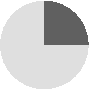
\includegraphics[width=12pt]{logos//circles//circle_onequarter.pdf}} }
\newcommand{\circc}{\raisebox{-0.25\height}{
\includegraphics[width=12pt]{logos//circles//circle_half.pdf}} }
\newcommand{\circd}{\raisebox{-0.25\height}{
\includegraphics[width=12pt]{logos//circles//circle_threequarter.pdf}} }
\newcommand{\circe}{\raisebox{-0.25\height}{
\includegraphics[width=12pt]{logos//circles//circle_full.pdf}} }

%%%%%%%%%%%%%%%%%%%%%%%%%%%%%%%%%%%
% Decrease page margins
%%%%%%%%%%%%%%%%%%%%%%%%%%%%%%%%%%%
\addtolength{\textheight}{0.7in}



\usepackage{mathtools}

\begin{document}

\newcommand{\TBD}{{\color{srldark}\textbf{TBD}}}
\newcommand{\TODO}[2]{{\color{srldark}\textit{TODO (#1): #2}}}

\newcommand{\criterion}[2]{#2 [#1]}
\newcommand{\crita}[2]{\criterion{A#1}{#2}}
\newcommand{\critk}[2]{\criterion{K#1}{#2}}
\newcommand{\critc}[2]{\criterion{C#1}{#2}}
\newcommand{\critt}[2]{\criterion{T#1}{#2}}
\newcommand{\critr}[2]{\criterion{R#1}{#2}}
\newcommand{\critp}[2]{\criterion{P#1}{#2}}

\maketitle
\pagebreak

\tableofcontents
\pagebreak

\section{Introduction}
\label{sec:introduction}

\section{Background}
\label{sec:background}

% explain GSM/3G connection setup
% (formal) syntax and semantics of traces
% which protocol layer are we considering?

% Explain IMSI catchers (Type x)
% Abbreviate messages
% Explain expressions - ranging from 0 - 1

\section{2G Security Metric}
\label{sec:2g_security_metric}

\section{3G Security Metric}
\label{sec:3g_security_metric}

\section{IMSI Catcher Detection Metric}
\label{sec:imsi_catcher_detection_metric}

\subsection{Attract}

This section covers detectable behavior that is geared towards attracting
mobile phones to register with an IMSI catcher instead of a regular network.

\subsubsection{\crita{1}{Different LAC/CID for the same ARFCN}}

The LAC/CID recently seen on an ARFCN suddenly changed.

\paragraph{Rationale}

An IMSI catcher may use the ARFCN of an existing BTS which has a weak signal in
the area the catcher operates. To force the MS into a location update, a LAC
different from all neighboring stations is chosen by the IMSI catcher.

The change of the LAC on a given ARFCN can be detected. Note, that for resource
efficiency, GSM reuses ARFCN in different geographic areas very frequently.
Hence, changes of the LAC/CID for a given ARFCN are specific to the geographic
location of the cell.

As associating an ARFCN/LAC/CID combination with a precise location reliably
can be challenging, a simpler approach should be taken. The ARFCN and LAC/CID
is recorded together with a time stamp. If the same ARFCN is used with a
different LAC/CID within a certain time frame, this is considered an attack.

\paragraph{False Positives}

Multiple BTS operating on the same ARFCN may be receivable in the same
locations, e.g. in elevated places. Furthermore, an operator may reconfigure
the cell to use a different LAC/CID.

\paragraph{Required Information}

The ARFCN ($ARFCN_{sc}$) and LAC/CID ($LAC_{sc}sc,CID_{sc}$) of the serving cell.

\paragraph{Expression}

$a_1 =
\begin{cases}
	0 & \text{if } id(ARFCN_{sc}) = \varnothing \vee id(ARFCN_{sc}) = LAC_{sc},CID_{sc} \\
	1 & \text{otherwise} \\
\end{cases}$

where $id$ is a database that maps the ARFCNs used during the last
$\Delta_{ARFCN}$ seconds to their respective LAC/CID.

The value of $\Delta_{ARFCN}$ has to be chosen small enough so that it is
unlikely to encounter the same ARFCN twice when the MS is moving quickly. This
could be approximated by the average distance of cells with the same ARFCN and
the maximum travel speed supported by GSM. We do not have this information
right now, so $\Delta_{ARFCN}$ must be configurable.

\paragraph{Source}

$LAC_{sc}$: Android API

\TODO{Jakob}{Find and document Android API call to retrieve $LAC_{sc}$.}

$CID_{sc}$: Android API

\TODO{Jakob}{Find and document Android API call to retrieve $CID_{sc}$.}

$ARFCN_{sc}$: ???

\TODO{Luca}{Find way to correlate ARFCN with the serving cell with Qualcomm DIAG.}

\subsubsection{\crita{2}{Inconsistent LAC}}

The LAC of the current base station differs from the LAC of many neighboring cells.

\paragraph{Rationale}

A MS will only perform a location update when changing to a different area,
i.e. a BTS with a different LAC. An IMSI catcher needs to force a location
update to be able to interact with the phone and derive the desired
information. Therefore, it must span a cell with a LAC different to all
neighboring cells, but with a much better signal strength than the other cells.
For an IMSI catcher announcing realistic neighboring cells, this difference
between the LAC of the serving cell and all neighboring cell can be detected.

\paragraph{False Positives}

Femto cells may or may not announce a LAC different from all their neighboring
cells. Their may be other special situations, like in-house cells where this is
the case.

\paragraph{Required Information}

Neighboring cell list $NL$ to derive $LAC_i$ values. The LAC of the serving
cell $LAC_{sc}$ and the LACs of the $k$ neighboring cells in the NL $LAC_i$.

\paragraph{Expression}

$a_2 =
\begin{cases}
	1 & \text{if } \displaystyle\sum_{i=1}^{k}
                        \begin{cases}
	                        1 & \text{if } LAC_i = LAC_{sc} \\
	                        0 & \text{otherwise}
                        \end{cases} = 0\\
        0 & \text{otherwise}
        \end{cases}
$

\paragraph{Source}

$LAC_{sc}$: Android API

\TODO{Jakob}{Find and document Android API call to retrieve $LAC_{sc}$.}
        
$NL$: Android API

\TODO{Jakob}{Find and document Android API call to retrieve $NL$.}
        
\subsubsection{\crita{3}{Only 2G available}}

No other technologies like 3G or 4G are available.

\paragraph{Rationale}

As of today, effective IMSI catchers are available for GSM only. Even the ones
advertised as 3G capable, rely on the fact that mobile phones fall back to GSM
in areas with no 3G available. To attack 3G or 4G capable phones, these
services are jammed by the IMSI catcher and an attack against GSM is mounted.
Having only GSM available should add to the overall score.

\paragraph{False Positives}

Bad network coverage. Areas without 3G and 4G.

\paragraph{Required Information}

List $RAT$ of radio access technologies currently available.

\paragraph{Expression}

$a_3 =
\begin{cases}
	0 & \text{if } 3G \in RAT \vee 4G \in RAT \\
	1 & \text{otherwise}
\end{cases}$

\paragraph{Source}

$RAT$: Android API or Android RIL

\TODO{Jakob}{Find and document Android API call or RIL call to retrieve $RAT$.}

\subsubsection{Score}

$A = \frac{a_1 + a_2}{2} + a_3$

\subsection{Keep}

Especially when a MS is tracked or tapped for a longer period of time, an IMSI
catcher must ensure it does not revert to a regular network cell. This section
describes detectable techniques IMSI catchers employ to keep mobile phones
registered.

\subsubsection{\critk{1}{No neighboring cells}}

The serving cell is not advertising any neighbor cells.

\paragraph{Rationale}

Active IMSI catchers which record voice and data will try to prevent an MS from
transitioning back to a regular cell. For that reason an IMSI catcher might
announce no neighboring cells such that the MS will use the cell spawned by the
IMSI catcher until its signal level is too low.

Note, that less suspicious options exist for an IMSI catcher to solve that
problem. It could announce a normal amount of neighboring cells, but choose
ARFCN not used by any BTS in that area.

\paragraph{False Positives}

Only few regular situations, like small islands with only a single call, are
thinkable where no neighboring cells may be announced.

\paragraph{Required Information}

Neighboring cell list $NL_{sc}$ of serving cell.

\paragraph{Expression}

$k1 =
\begin{cases}
	1 & \text{if } \left|NL_{sc}\right| = 0 \\
	0 & \text{otherwise}
\end{cases}$

% \FIXME{Extract and graph the number of neighboring cells for all cells in the
% GSMmap sample set to get the function $p(n)$ expressing the likelihood of a
% cell to announce $n$ neighboring cells.}

\paragraph{Source}

$NL_{sc}$: Android API

\TODO{Jakob}{Find and document Android API call to retrieve $NL_{sc}$.}

\subsubsection{\critk{2}{High cell reselect offset}}

The cell reselect offset is high.

\paragraph{Rationale}

The goal of announcing a large CELL RESELECT OFFSET is similar to K1. The CELL
RESELECT OFFSET is used to calculate the reselection criterion C2. Together
with the path loss criterion parameter C1 it is "used to ensure that the MS is
camped on the cell with which it has the highest probability of successful
communication on uplink and downlink." \cite[6.4]{gsm0508}

In cases where an IMSI catcher e.g. announces real, available neighboring
cells, it might choose to announce a CELL RESELECTION OFFSET that would require
the signal quality of any neighboring cell to be impossibly good to consider it
as an alternative to the cell spawned by the IMSI catcher. This makes the MS
camp on that cell until the desired information has been collected.

% \TODO{Add cell reselection formula to explain the above statement.}

% Explanation by Andreas Eversberg on Thu Jan 26 17:28:30 CET 2012
% (CatcherCatcher mailing list):
%
% - a catcher uses a high CRO (cell reselection offset). an offset up to
% 126 db makes a neighbour cell (catcher) +126 db "better" than the actual
% receive level from the catcher. a better cell is then selected by the
% phone, because "rx(cather)+CRO > rx(regual cell)+CRH". (CRH is used when
% changing location areas. it is generally set to 6db.)

\paragraph{False Positives}

Networks may announce a high CELL RESELECTION OFFSET in areas with poor
coverage.

% \TODO{Check what exactly is done with C1/C2/CELL RESELECTION OFFSET/TEMPORARY OFFSET}

\paragraph{Required Information}

Cell reselection parameter $CRO_{sc}$ for the serving cell from BCCH/SI3.

\paragraph{Expression}

$k2 =
\begin{cases}
	0 & CRO_{sc} < CRO_{max}\\
	1 & \text{otherwise}
\end{cases}$

where $CRO_{max}$ is the value still considered normal for the CRO. As a
suitable value for is not yet known, this value must be configurable.

\paragraph{Source}

$CRO_{sc}$: Qualcomm DIAG, BCCH/SI3, Cell database field \verb|cell_info.cro|

\TODO{Luca}{Store to cell info database.}

\TODO{Luca}{We cannot distinguish serving cell SI3 information from neighboring
cell SI3 information. Find way to correlate ARFCN with the serving cell with
Qualcomm DIAG.}

\subsubsection{Score}

$K = k_1 + k_2$

\subsection{Collect}

This section describes criteria related to the information collection process
of an IMSI catcher. This includes actions necessary to break encryption as well
as direct information gathering.

\subsubsection{\critc{1}{Encryption Downgrade}}

After using an encryption algorithm with a cell previously, encryption got
downgraded to a weaker algorithm.

\paragraph{Rationale}

Encryption may be disabled completely (A5/0) or limited to a deliberately
weakened algorithm (A5/2) due to legal restrictions in some countries.
Furthermore, an operator may not yet have the technical capabilities to use the
more secure A5/3 algorithm in all of his cells in favor of the broken A5/1 one.

If a weaker encryption algorithm is observed for the same cell at a later time,
this may be an indication for an attacker forcing the MS into an encryption
mode that she can attack (more easily). The most likely situation for an active
IMSI catcher is a downgrade to A5/0, i.e. null encryption. A downgrade from
A5/3 to A5/1 is expected to be rare, as for an active attacker it is much
easier to disable encryption all together instead of cracking A5/1.

This metric is relevant and applicable only when an existing LAC/CID is reused
for an IMSI catcher. This is not very common, though, as IMSI catchers usually
create a new cell with different LAC to force the MS into a location update.
However, if an encryption downgrade happens, this is a very strong sign for an
attack.

\paragraph{False Positives}

An operator may mis-configure some of its base stations to use a weaker
encryption algorithm. In rare cases A5/0 transaction are observed, most likely
caused by hardware faults.

%\FIXME{May A5/0 transactions be caused by mobiles not supporting / refusing to perform encryption?}

\paragraph{Required Information}

A record of the strongest encryption algorithm that was observed for a given
cell ($A_{best}$). The CIPHER MODE COMMAND to extract the encryption algorithm
currently in use ($A$).

\paragraph{Expression}

$c_1 =
\begin{cases}
	1 & \text{if } s(A) < s(A_{best}) \\
	0 & \text{otherwise}
\end{cases}$

where $s(a)$ -- the strength of the encryption algorithm $a$ -- is defined as

$s(A5/0) < s(A5/2) < s(A5/1) < s(A5/3)$.

\paragraph{Source}

$A$: Transaction database field \verb|session_info.cipher|

\subsubsection{\critc{2}{Delayed CIPHER MODE COMPLETE acknowledgement}}

CIPHER MODE COMPLETE messages may be acknowledged by an IMSI Catcher with
significant delay.

\paragraph{Rationale}

When an active IMSI catcher mounts an attack against the A5/1 algorithm it
takes a significant amount of time to break the encryption (up to a couple of
seconds). During this period, the CIPHER MODE COMPLETE message is retransmitted
by the MS until an acknowledgment is received, assuming a previous message has
not reached the BTS. Both can be detected, the increase delay and a higher
retransmission count.

\paragraph{False Positives}

Lost CIPHER MODE COMPLETE packets due to bad network reception.

\paragraph{Required Information}

Time stamp of the first CIPHER MODE COMPLETE message ($t_{CMCP_0}$) and the
last CIPHER MODE COMPLETE message ($t_{CMCP_l}$).

\paragraph{Expression}

$c_2 =
\begin{cases}
	0 	&  \text{if } t_{CMCP_l} - t_{CMCP_0} < \Delta_{CMCP} \\
	1       &  \text{otherwise}
\end{cases}$

where $\Delta_{CMCP}$ is the maximum time for accepting a CIPHER MODE COMPLETE
message considered normal for a network. We do not have this information right
now, so $\Delta_{CMCP}$ must be configurable.

% \TODO{Graph the delays between CIPHER MODE COMPLETE and first encrypted
% message based on GSMmap data over all data sets. Approximate a formula of that
% empiric data and invert and scale it such that abnormally long and abnormally
% short delays yield a score of 1. The resulting formula is $p(t)$.}

\paragraph{Source}

$t_{CMCP_0}$: Transaction database field \verb|session_info.cipher_comp_first|

$t_{CMCP_l}$: Transaction database field \verb|session_info.cipher_comp_last|

\subsubsection{\critc{3}{CIPHER MODE COMMAND message without IMEISV}}

In the CIPHER MODE COMMAND message from the network no IMEISV was requested.

\paragraph{Rationale}

The absence of an IMEISV makes the CIPHER MODE COMPLETE message -- the response
to the CIPHER MODE COMMAND message -- fully predictable. This enables an IMSI
catcher to mount a known-plaintext attack against the crypto algorithm.
Consequently, IMSI catchers may direct the MS to omit the IMSISV in its
response.

\paragraph{False Positives}

Not requesting the IMEISV is normal behaviour in some networks, as the IMEI may
be retrieved through a subsequent IDENTITY REQUEST at any later time.

\paragraph{Required Information}

The value of the Cipher Response field (CR) of the last CIPHER MODE COMMAND
message $CR$ (cf. \cite[10.5.2.10]{gsm0408}).

\paragraph{Expression}

$c_3 =
\begin{cases}
	0       & \text{if } CR = 1 \\
	1	& \text{otherwise}
\end{cases}$

% where $p_{IMEISV}$ is the likelihood that operators request the IMEISV in their
% normal CIPHER MODE COMMAND messages.

% \TODO{From the GSMmap sample set, calculate the likelihood $p_{IMEISV}$ that
% the IMEISV will be requested during normal operation.}

\paragraph{Source}

$CR$: Transaction database field \verb|session_info.cmc_imeisv|

\subsubsection{\critc{4}{ID requests during location update}}

The network queries identity information (like IMSI and IMEI) after a LOCATION
UPDATE REQUEST and then rejects that request.

\paragraph{Rationale}

This is a fingerprint of a type 1 IMSI catcher, which ends the transaction as
soon as the identity of the MS has been recorded. In a sound network setup, one
can assume that an identity request only happens when encryption is in place,
i.e. after a CIPHER MODE COMPLETE.

A MS has to perform a cell reselection when a LOCATION UPDATE REQUEST has been
rejected with a "location area not allowed". This may be used by the IMSI
catcher to force the MS so select a different cell after the desired
information was collected.

\paragraph{False Positives}

Unknown.

\paragraph{Required Information}

Whether the IMSI was requested \emph{before} ciphering ($ID_{IMSI}$) and
whether IMEI was requested \emph{before} ciphering ($ID_{IMEI}$).

% The type of LOCATION UPDATE REQUEST (attach, periodic or normal) $T_{LURQ}$
% and the cause of the LOCATION UPDATE REJECT $C_{LURJ}$.

\paragraph{Expression}

$c_4 =
\begin{cases}
	1 	& \text{if } ID_{IMSI} \wedge ID_{IMEI} \\
	0.7     & \text{if } ID_{IMSI} \oplus ID_{IMEI} \\
	0       & \text{otherwise}
\end{cases}$

\paragraph{Source}

$ID_{IMSI}$: Transaction database field \verb|session_info.iden_imsi_bc|

$ID_{IMEI}$: Transaction database field \verb|session_info.iden_imei_bc|

\subsubsection{Score}

$C = c_1 + c_2 + c_3 + c_4$

\subsection{Track}

Besides the collection of information, IMSI catchers are used to determine the
location of a MS or to just detect the presence of a MS in the range of the
IMSI catcher. This section outlines detectable side-effects of this process.

\subsubsection{\critt{1}{Low registration timer}}

The initial value of the registration timer T3212 is low.

\paragraph{Rationale}

The registration timer T3212 controls the interval a MS performs a periodic
LOCATION UPDATE, i.e. one that is performed regularly when the location area of
the MS does not change. The T3212 of an MS is initialized from the time-out
value in the \emph{Control Channel Description} which is broadcast as part of
SI3 on the serving cells BCCH. It can be set at a granularity of decihours
(6~minutes) and supports a maximum value of 25.5 hours (255~decihours). The
value of 0 disables periodic location updates completely.

An IMSI catcher might broadcast an initialization value for the registration
timer that causes the phone to updates its location with the catcher very
often, e.g. every 6 minutes. This allows for rather precise presence tracking.

\paragraph{False Positives}

Unknown.

\paragraph{Required Information}

Time-out initialization value for T3212 ($T3212_0$) from the \emph{Control
Channel Description} part of the serving cells SI3.

\paragraph{Expression}

$t1 =
\begin{cases}
	1 	& \text{if } T3212_0 < T3212_{min} \\
	0       & \text{otherwise}
\end{cases}$

where $T3212_{min}$ is the minimum value of $T3212$ considered "normal". We do
not have this information right now, so $T3212_{min}$ must be configurable.

\paragraph{Source}

$T3212_0$: Qualcomm DIAG, BCCH/SI3, Cell database field \verb|cell_info.t3212|

\TODO{Luca}{Store to cell database.}

\TODO{Luca}{We cannot distinguish serving cell SI3 information from neighboring
cell SI3 information. Find way to correlate ARFCN with the serving cell with
Qualcomm DIAG.}

\subsubsection{\critt{3}{Paging without transaction}}

The MS is paged without entering a transaction.

\paragraph{Rationale}

Paging by IMSI and subsequently releasing the transaction without SMS or call
data being transmitted may be a pattern of a tracking IMSI catcher trying to
detect whether a particular user is in the area of the catcher.

\paragraph{False Positives}

A similar pattern occurs when a MS is called, but the caller releases the call
quickly enough such that the MS is paged, but no ALARM is signaled.

\paragraph{Required Information}

$M_i$ indicates whether message of type $i$ was received in a transaction:

\begin{tabular}{ll}
\hline
$M_{CR}$   & RR CHANNEL RELEASE \\
$M_{AR}$   & MM AUTHENTICATION REQUEST \\
$M_{IR}$   & IDENTITY REQUEST \\
$M_{CM}$   & RR CIPHER MODE COMMAND \\
$M_{SD}$   & SMS-DELIVER \\
$M_{SU}$   & CC SETUP \\
$M_{PRS}$  & PAGING RESPONSE \\
$MI_{PRS}$ & Mobile identity type used in PAGING RESPONSE \\
\hline
\end{tabular}

\paragraph{Expression}

$t3 =
\begin{cases}
	1 & \text{if } MI_{PRS} = \text{"IMSI"} \wedge M_{PRS} \wedge M_{CR} \wedge \neg M_{AR} \wedge \neg M_{IR} \wedge \neg M_{CM} \wedge \neg M_{SD} \wedge \neg M_{SU} \\
	0 & \text{otherwise}
\end{cases}$

\paragraph{Source}

$MI_{PRS}$: Transaction database field \verb|session_info.paging_mi|

$M_{PRS}$: Transaction database field \verb|session_info.mobile_term|

$M_{CR}$: Transaction database field \verb|session_info.t_release|

$M_{AR}$: Transaction database field \verb|session_info.auth|

$M_{IR}$: Transaction database fields \verb|session_info.iden_im{e,s}i_{a,b}c|

$M_{CM}$: Transaction database field \verb|session_info.cipher > 0|

$M_{SD}$: Transaction database field \verb|session_info.sms_presence|

$M_{SU}$: Transaction database field \verb|session_info.call_presence|

\subsubsection{\critt{4}{Orphaned traffic channel}}

A traffic channel is assigned, but no call control state is entered or text
message received for a long time.

\paragraph{Rationale}

When a traffic channel is assigned, the MS is constantly sending (idle
messages) until the channel is released. This constant transmission can be
exploited by an IMSI catcher to perform a more accurate localization of the MS.

\paragraph{False Positives}

Unknown.

\paragraph{Required Information}

$M_i$ indicates whether message of type $i$ was received in a transaction and
$t_i$ designates the timestamp message of type $i$ was received:

\begin{tabular}{ll}
\hline
$t_{TR} $ & Transaction duration \\
$M_{AC} $ & RR ASSIGNMENT COMPLETE for TCH \\
$M_{CR} $ & RR CHANNEL RELEASE \\
$M_{AR} $ & MM AUTHENTICATION REQUEST \\
$M_{IR} $ & IDENTITY REQUEST \\
$M_{CM} $ & RR CIPHER MODE COMMAND \\
$M_{SD} $ & SMS-DELIVER \\
$M_{SU} $ & CC SETUP \\
$M_{PRS}$ & PAGING RESPONSE \\
\hline
\end{tabular}

\TODO{Luca}{Check this list for correctness and completeness.}

\paragraph{Expression}

$t4 =
\begin{cases}
	1 & \text{if } (M_{AC} \vee M_{PR}) \wedge M_{CR} \wedge \neg M_{AR} \wedge \neg M_{IR} \wedge \neg M_{CM} \wedge \neg M_{SD} \wedge \neg M_{SU} \wedge (t_{TR} > \Delta_{TCH}) \\
	0 & \text{otherwise}
\end{cases}$

where $\Delta_{TCH}$ is the maximum value an idle traffic channel is considered
"normal". We do not have this information right now, so $\Delta_{TCH}$ must be
configurable.

\paragraph{Source}

$t_{TR}$: Transaction database field \verb|session_info.duration|

$M_{AC}$: Transaction database

\TODO{Luca}{Add new field for ASSIGN COMPLETE}

$M_{CR}$: Transaction database field \verb|session_info.t_release|

$M_{AR}$: Transaction database field \verb|session_info.auth|

$M_{IR}$: Transaction database fields \verb|session_info.iden_im{e,s}i_{a,b}c|

$M_{CM}$: Transaction database field \verb|session_info.cipher > 0|

$M_{SD}$: Transaction database field \verb|session_info.sms_presence|

$M_{SU}$: Transaction database field \verb|session_info.call_presence|

\subsubsection{\critt{7}{MS sends on high power}}

The MS sends on high power.

\paragraph{Rationale}

An IMSI catcher may instruct the MS to send at high power to maximize the range
of the catcher.

\paragraph{False Positives}

Bad reception, e.g. in rural areas.

\paragraph{Required Information}

Current transmission level $TX$.

\paragraph{Expression}

$t6 =
\begin{cases}
	1 & \text{if } TX > TX_{max} \\
	0 & \text{otherwise}
\end{cases}$

where $TX_{max}$ is the maximum $TX$ value that is considered "normal". We do
not have this information right now, so $TX_{max}$ must be configurable.

\paragraph{Source}

$TX$: Android?

\TODO{Jakob}{Find and document Android API call or Android RIL call to retrieve $TX$.}

\subsubsection{Score}

$T = t_1 + t_3 + t_7$

\subsection{Reject}

After an MS was registered with an IMSI catcher, the operator of the device may
want to disassociate certain phones from the catcher while leaving others under
surveillance. This section covers detectable traces of this process.

\subsubsection{\critr{1}{Inconsistent neighbor list}}

The neighbor list of most neighboring cells does not contain serving cell.

\paragraph{Rationale}

In a regular network one can assume that the majority of neighboring cells of
the current serving cell also announce the current cell as one of their
neighboring stations. 

A strategy of an IMSI catcher to prevent an MS that was already connected to
register again, is to send a neighbor list over the BCCH that contains only
neighboring cells which do \emph{not} have the ARFCN of the IMSI catcher in
their own neighbor list \cite[0027]{bott2000verfahren}. When the MS selects one of
those neighboring cells, it will not consider the IMSI catcher at least for the
next cell reselection.

\paragraph{False Positives}

Unknown.

\paragraph{Required Information}

Neighbor lists of all $k$ neighboring cells $NL_i$. ARFCN of the serving cell
$ARFCN_{sc}$.

\paragraph{Expression}

$r1 =
\begin{cases}
	1 & \text{if } \left(\frac{1}{k}\displaystyle\sum_{i=1}^{k}
                                \begin{cases}
	                                1 & \text{if } ARFCN_{sc} \in NL_i \\
	                                0 & \text{otherwise}
                                \end{cases}\right) < NL_{min} \\
        0 & \text{otherwise}
        \end{cases}
$

where $NL_{min}$ is the minimum fraction of neighboring cell neighbor lists
containing the serving cells $ARFCN$. We do not have this information right
now, so $NL_{min}$ must be configurable.

\paragraph{Source}

$NL_i$: Qualcomm DIAG, BCCH/SI2

\TODO{Luca}{Add to parser and transaction database.}

\TODO{Luca}{We cannot distinguish serving cell SI2 information from neighboring
cell SI2 information. Find way to correlate ARFCN with the serving cell with
Qualcomm DIAG.}

\TODO{Luca}{Which DB field?}

$ARFCN_{sc}$: ???

\TODO{Luca}{Find way to correlate ARFCN with the serving cell with Qualcomm
DIAG.}

\subsubsection{\critr{2}{High number of paging groups}}

The cell is configured in a way that maximizes the number of paging groups.

\paragraph{Rationale}

When an IMSI catcher uses the technique described in
\cite[0021]{bott2000verfahren} to force the MS back into a regular network,
invalid data is sent on the PCH of the respective paging group of that MS until
the MS performs a cell reselection. This has the side effect that any other MS
on the same paging group also selects a different cell. Hence, the cell spawned
by an IMSI catcher using this technique will try to maximize the number of
paging groups ($N$) in that cell to increase the granularity at which MSes can
be disconnected.

${N} = (9 - {\text{BS\_AG\_BLKS\_RES}} - 6\times {\text{BS\_CCCH\_SDCCH\_COMB}})\times {\text{BS\_PA\_MFRMS}}$

\paragraph{False Positives}

Unknown.

\paragraph{Required Information}

BS\_AG\_BLKS\_RES, BS\_CCCH\_SDCCH\_COMB and BS\_PA\_MFRMS

\paragraph{Expression}

$r2 =
\begin{cases}
	1 & \text{if } N > N_{norm} \\
        0 & \text{otherwise}
        \end{cases}
$

where $N_{norm}$ is the maximum number of paging groups considered "normal". We
do not have this information right now, so $N_{norm}$ must be configurable.

\paragraph{Source}

BS\_AG\_BLKS\_RES: BCCH/SI3, Cell database field \verb|cell_info.agch_blocks|

BS\_CCCH\_SDCCH\_COMB: BCCH/SI3, Cell database field \verb|cell_info.combined|

BS\_PA\_MFRMS: BCCH/SI3, Cell database field \verb|cell_info.pag_mframes|

\subsubsection{Score}

$R = r_1 + r_2$

\subsection{Overall Score}

$S = A + K + C + T + R$

$Catcher =
\begin{cases}
	\text{red}   & \text{if } M_{red} \leq S \\
        \text{amber} & \text{if } M_{amber} \leq S < M_{red} \\
        \text{green} & \text{if } S < M_{amber} \\
\end{cases}
$

where $M_{amber}$ and $M_{red}$ are the respective margins for the traffic
light classification of the overall score $S$ with $M_{amber} < M_{red}$. We do
not have this information right now, so $M_{amber}$ and $M_{red}$ must be
configurable.

\bibliographystyle{plain}
\bibliography{bibliography}

\end{document}
